\section{Computing Critical Points and Their Connectivity}

This section presents two important algorithms required to compute the critical points of an image and their connectivity. The first algorithm detects both the minima and watershed pixels and is called $min\_watershed\_detector(I, \sigma)$ where $I$ is the image and $\sigma$ is a smoothing parameter. Note that the same function can be used to detect maxima and watercourse by inverting the image. Its implementation is very similar to the standard watershed transform which works as follows \cite{WatershedWiki}: A set of seed pixels is selected and given different labels. The pixels surrounding the seed pixels are inserted into a priority queue where the pixel priority is based on how low its intensity value is. Then, the pixel with highest priority is chosen. If its already labeled neighbors have the same label, it is given that label. Otherwise, it is kept unlabeled. Then, all unlabeled neighboring pixels are added to the priority queue. The algorithm goes on like this until the priority queue becomes empty. At the end, the labeled pixels are the basins while the unlabeled ones correspond to watershed pixels. The key differences of our algorithm from the traditional one are: \textit{(i)} There is no need for an apriori detection of minima (the seed pixels) since the detection is an integral part of the algorithm; \textit{(ii)} The algorithm keeps track of the identities of the minima giving rise to each watershed pixel. 
Note that $min\_watershed\_detector(I, \sigma)$ may also be implemented  by separating the detection of extended minima\footnote{An extended minima is a connected cluster of pixels with the same intensity value surrounded by higher intensity pixels. An implementation of this is MATLAB's $imregionalmin$.} as a first, separate stage, and then using the traditional watershed transform to label pixels either as the watershed pixels or basins. Next, using the basin labels that are neighbors to each watershed pixel, the identities of the minima giving rise to each watershed pixel can be found\footnote{Not sure if this would be identical to what we compute in our algorithm.}.

The second algorithm, $TAG\_detector(I, \sigma)$, aims to find saddles and then connect all the critical points, namely, minima, maxima and saddle points in a graph structure called Topological Appearance Graph (TAG). It uses the minima and watershed pixels detected by the $min\_watershed\_detector(I, \sigma)$ and the maxima and watercourse pixels detcted by the $min\_watershed\_detector(-I, \sigma)$. Since our definition of saddles is the intersection of watershed and watercourse lines, it utilizes the watershed/watercourse pixels to localize the saddles. In addition, since the ids of minima/maxima giving rise to watershed/watercourse pixels are known, the algorithm is able to establish connections between all the critical points which results in the TAG of the input image $I$. 
\\

\begin{figure}
\centering
\includegraphics[width=.45\textwidth]{img/self-collision.png}
\caption{A self-colliding basin. This case is currently ignored by the algorithm.}
\label{fig:selfcollision}
\end{figure}

\noindent \textbf{function $min\_watershed\_detector(I, \sigma)$:}
\\

\textbf{Summary:} The goal is to find all the minima and watershed pixels with the ids of the basins (minima) who gave rise to them. In order to achieve this, the intensity values in the image are first sorted from low to high. As in the traditional watershed transform, the intensity is thought of as rising water levels. Then, we visit each water level in increasing order and find out which pixels have just been covered with water (we call them \textit{event pixels}). Next, we classify each connected component of the event pixels in one of three classes: \textit{(i)} minimum, \textit{(ii)} watershed pixel or \textit{(iii)} basin growth (all pixels of a connected component are given the same label\footnote{Prof. Kimia asked me if it is possible to assign the pixels of a connected component to different classes. For example, can some part of the connected component be a basin growth while the other parts are watershed pixels? I do not know the answer. \todo{We need an explanation.}}). Note that if the connected component has more than one pixel, the result is an \textit{extended} minimum, \textit{extended} watershed or \textit{extended} basin growth. Once all the water levels are visited, the algorithm stops. For the detailed algorithm steps, see below:
\\

\textbf{Failure mode:} Self-collisions are not handled (Figure \ref{fig:selfcollision}). Some watershed pixels may not be detected which will cause the algorithm to miss the saddles due to self-collisions. 
\\

\noindent \textbf{Input:} 
\begin{itemize}
\item Image $I$
\item $\sigma$ for smoothing
\end{itemize}

\noindent \textbf{Output:} 
\begin{itemize}
\item $ws$: the unorganized list of watershed pixels
\item $mins$: the minima of $I$
\item $ws\_basins$: ids of the minima giving rise to each watershed pixel
\end{itemize}
\textbf{Local variables:}
\begin{itemize}
\item $i$: the index of the loop visiting the sorted water levels.
\item $sorted\_I$: the sorted array of unique intensity values in $I$.
\item $Water\_Level$: the level of the rising water.
\item $Label\_prev$: an image with the same size as $I$. Each pixel holds the basin id assigned to it before visiting the current water level. 0 means ``not assigned" yet.
\item $Label\_curr$: an image with the same size as $I$. Each pixel holds the basin id assigned to it after visiting the current water level. 0 means ``not assigned" yet.
\item $num\_min$: the number of minima.

\end{itemize}

\begin{figure}
\centering
\includegraphics[width=.85\textwidth]{img/boundary.png}
\caption{In this example, the blue triangles are the maxima, the blue circles are the minima, the red x's are the watershed, the green x's are the watercourse and the yellow x's are the intersection of the watershed and watercourse pixels. Observe the image boundary pixels after processing the image with mirror reflection padding. Most of the boundary pixels are either critical points or watershed/watercourse pixels. The only exception happens when there is a direct transition from a minimum to maximum along the boundary.}
\label{fig:reflectionboundary}
\end{figure}

\begin{figure}
\centering
\subfloat[Watershed creation. Since the event pixel is adjacent to two separate basins, it is classified as a watershed pixel.]{\label{fig:wscreation}\includegraphics[height=.25\textheight]{img/eventpix/watershedcreation.png}}\;
\subfloat[Watershed growth. The orange pixels are the previously classified watershed pixels and the red, green, cyan and yellow regions correspond to 4 seperate basins. Since the event pixel is only adjacent to the existing watershed pixels, it is classified as a watershed pixel as well.]{\label{fig:wsgrowth}\includegraphics[height=.25\textheight]{img/eventpix/watershedgrowth.png}}\\
\subfloat[Basin creation. Since the event pixel is not adjacent to any watershed or basin pixel, it is classified as a new basin (minimum).]{\label{fig:basincreation}\includegraphics[height=.25\textheight]{img/eventpix/basincreation.png}}\;
\subfloat[Basin growth. Since the event pixel is adjacent to only one basin, it is just a part of that basin. Thus, it is classified as a basin pixel.]{\label{fig:basingrowth}\includegraphics[height=.25\textheight]{img/eventpix/basingrowth.png}}
\caption{Event pixel classification examples. The white pixels are the event pixels to be classified.}
\label{fig:eventpixclasses}
\end{figure}

\textbf{Algorithm:}
\begin{enumerate}
	\item Pad the image boundary using the mirror reflection of the image. I use $(7\sigma-1)/2$ pixels for padding each side. The motivation for using mirror reflection instead of constant value continuation is that mirror reflection causes most of the boundary pixels to become either critical points or watershed/watercourse pixels. This is violated only when there is a direct transition from a minimum to maximum along the boundary, \ie the absence of a saddle point on the boundary to form a watershed/watercourse line. See Figure \ref{fig:reflectionboundary}.

	\item Smooth the padded image with a Gaussian with standard deviation $\sigma$. \footnote{This step may not be required in the future, as structural smoothing after graph construction may be more meaningful.}

	\item Sort all the intensity values in the image in ascending order to create $sorted\_I$.
	\item Start a loop with $i = 1$, $Label\_prev$ = initially all 0's and $num\_min = 0$ 
	\begin{enumerate}[i.]
		\item Set $Water\_Level$ = $sorted\_I[i]$.
		\item Compute the mask $Mask\_curr$: If the image intensity $\leq Water\_Level$, the mask is set to $-1$. Otherwise, it is set $0$. The reason for using $-1$ instead of $1$ will become clear shortly.
		\item $Label\_curr = Mask\_curr$.
		\item Copy non-zero labels from the previous iteration ($Label\_prev$) into $Label\_curr$. So, now $Label\_curr$ has the same labels as $Label\_prev$, but additionally it also has pixels labeled as $-1$ which correspond to new pixels covered with water, the so-called ``event pixels" which will correspond to either minima creation, watershed creation or basin growth.
		\item Classify each connected component of event pixels as ``min", ``watershed" or ``basin growth".
		\begin{enumerate}[(a)]
			\item \textbf{[watershed creation]} Figure \ref{fig:wscreation}. It is a ``watershed" if it touches at least 2 separate regions with non-zero labels. Add each pixel of the component to $ws$. Add the ids of the basins participating in the collision to $ws\_basins$. In this way, we always know which minima give rise to which watershed pixels.	
			\begin{enumerate}
				\item \textbf{[watershed growth]} Figure \ref{fig:wsgrowth}. \todo{Added this condition recently, not sure about its correctness.} It is a ``watershed" if it is surrounded by 0s in $Label\_curr$, but at least one of the surrounding pixels has been labeled as ``watershed". This case does not happen frequently, but it can still happen. However, I am not sure if this is the best way to handle it. In order to handle this case more properly, the watershed pixels can be represented as $-2$ in $Label\_curr$ and $Label\_prev$.
			\end{enumerate}		

			\item \textbf{[basin creation]} Figure \ref{fig:basincreation}. It is a ``min" if it is surrounded by 0s in $Label\_curr$ and none of the surrounding pixels has been labeled as ``watershed". Either fit a surface to find the subpixel position or take the centroid of the component and add it to $mins$. $num\_min = num\_min + 1$.		
			

			\item \textbf{[basin growth]} Figure \ref{fig:basingrowth}. It is a ``basin growth" if it touches only one region with a non-zero label. 
		\end{enumerate}
		
		\item Update $-1$s in $Label\_curr$ with appropriate labels (use label $-2$ for watershed creation, label $num\_min$ for basin creation and the label of the growing basin for basin growth)

		\item $Label\_prev = Label\_curr$.

		\item $i = i + 1$.
		
		\item Exit the loop if all the water-levels have been visited.
	\end{enumerate}
	5) Return $mins$, $ws$ and $ws\_basins$.\\\\
\end{enumerate}



\noindent \textbf{function $TAG\_detector(I, \sigma)$:}
\\

\textbf{Summary:} The graph connecting the critical points can only connect saddles to other critical points, \ie, the only connection of maximum and minimum is to saddle point and not to other maximum or minimum. So, we first compute the minima/maxima and watershed/watercourse pixels. Then, based on our definition of saddles, we intersect the watershed and watercourse pixels and find the saddle candidates. Next, we classify each candidate either as saddle or as a series of saddle points connected as a chain. Finally, we connect all the saddle points to minima, maxima and other saddles based on the identities of minima/maxima giving rise to each watershed pixel. This generates the TAG of $I$. 
\\

\textbf{Failure mode:} I do not have a generalized rule to find saddle-saddle connections. So, the saddle-saddle connections are ignored which causes the algorithm to create incorrect links in the TAG. \todo{Show examples.}
\\

\noindent \textbf{Input:} 
\begin{itemize}
\item Image $I$
\item $\sigma$ for smoothing
\end{itemize}

\noindent \textbf{Output:}
\begin{itemize}
\item $mins$: the list of minima of $I$
\item $maxs$: the list of maxima of $I$
\item $saddles$: the list of saddle points of $I$
\item $saddle\_links$: the ids of the minima/maxima/saddle points connected to each saddle. It corresponds to the TAG of $I$.
\end{itemize}

\noindent \textbf{Local variables:}
\begin{itemize}
\item $ws$: the unorganized list of watershed pixels of $I$
\item $wc$: the unorganized list of watercourse pixels of $I$
\item $ws\_basins$: ids of the minima giving rise to each watershed pixel
\item $wc\_hills$: ids of the maxima giving rise to each watercourse pixel
\item $ws\_wc\_common$: common pixels of $ws$ and $wc$
\item $saddle\_candidates$: the list of connected components in $ws\_wc\_common$
\end{itemize}

\begin{figure}
\centering
\subfloat[]{\includegraphics[height=.32\textheight]{img/connsaddle1.png}}\;
\subfloat[]{\includegraphics[height=.32\textheight]{img/connsaddle5.png}}\\
\subfloat[]{\includegraphics[height=.24\textheight]{img/connsaddle3.png}}\;
\subfloat[]{\includegraphics[height=.24\textheight]{img/connsaddle6.png}}\\
\subfloat[]{\label{fig:saddlecandidates}\includegraphics[width=.95\textwidth]{img/connsaddle4.png}}
\caption{In these examples, the blue triangles are the maxima, the blue circles are the minima, the red x's are the watershed, the green x's are the watercourse and the yellow x's are the intersection of the watershed and watercourse pixels. The yellow chains are the examples of the cases where I think the saddle-saddle connections occur. Note that there are other yellow groups with 1 or 2 pixels, too. Those are the examples of isolated saddle points. Do not confuse them with the saddle chains.}
\label{fig:connsaddle}
\end{figure}

\noindent \textbf{Algorithm:}
\begin{enumerate}
	\item Call $min\_watershed\_detector(I, \sigma)$  to compute $ws$, $mins$ and $ws\_basins$ 

	\item Call $min\_watershed\_detector(-I, \sigma)$ to compute $wc$, $maxs$ and $wc\_hills$ 

	\item Find the intersection of $ws$ and $wc$ and store these pixels in $ws\_wc\_common$. These are saddle points either as isolated saddle points or as chains of saddle points (See Figure \ref{fig:saddlecandidates}). Keep track of the ids in $ws\_basins$ and $wc\_hills$ and associate them with each pixel in $ws\_wc\_common$.

	\item Find the connected components in $ws\_wc\_common$ and store them in $saddle\_candidates$. 

	\item Classify and store each connected component in $saddle\_candidates$ as follows:
	\begin{enumerate}[i.]
		\item \label{item:regularsaddle} If all the pixels of the component have the same min and max ids according to their entries in $ws\_basins$ and $wc\_hills$, fit a quadratic surface to the entire component, find its subpixel critical point and add it to $saddles$. \footnote{Subpixel computation part is disabled, but there is code to accomplish that. For now, I just average the coordinates of the pixels that belong to the component.} 
		\item \label{item:connsaddle} Otherwise, this may imply that this component corresponds to at least two saddle points connected by saddle-saddle links. \footnote{I haven't been able to generalize this case, so it does not work for now.} See Figure \ref{fig:connsaddle} for examples of this case.
	\end{enumerate}

	\item Compute $saddle\_links$ (ids of minima/maxima/saddle points connected to each saddle) based on the component classification results. Basically, use the entries in $ws\_basins$ and $wc\_hills$ if it is classified according to Step \ref{item:regularsaddle}. \todo{Use the connected saddle information if it is classified according to Step \ref{item:connsaddle}.}

	\item Return $mins$, $maxs$, $saddles$ and $saddle\_links$. 
\end{enumerate}



